\section{Security Architectures}\label{sec:Security_Architectures}
\begin{questions}
\question{} Describe what constitutes a security architecture and give some examples.
  \begin{solution}
    A Security Architecture has graphical and textual representations of a security system.
    It includes relations, trust levels, trust relationships, and interfaces between different parts of the system.
    It also has security and system boundaries to delimit different parts of the system that have various properties.
  \end{solution}

\question{} The Sherwood Applied Business Security Architecture (SABSA) consist of 5 layers and one cross layer.
  \begin{parts}
  \part{} Describe the different layer views and list the names of the different layers.
    \begin{solution}
      \begin{enumerate}[noitemsep]
      \item Contextual Security Architecture is the view the business has of the system.
        It is quite similar to the Security Requirements.
      \item Conceptual Security Architecture is the highest-level view that an engineer can have of the system.
        This includes the general breakdown into secure portions of a system.
      \item Logical Security Architecture is the next level, that deals with data and its logical flows.
        Here, the way that data and its logical propagation are safeguarded is first developed.
      \item Physical Security Architecture is the 3rd design level.
        Here, the specific high-level security requirements and previous security architecture levels are combined to choose what needs to be done to secure the data.
      \item Component Security Architecture is the lowest level of the SABSA Security Architecture.
        Here, the actual protocols, standards, and hardware are chosen.
      \item Security Service Management Architecture is the ``cross layer''.
        It is concerned with how to maintain the system and its security.
      \end{enumerate}
    \end{solution}

  \part{} Give examples of questions the different SABSA architecture views are supposed to answer.
    \begin{solution}
      \begin{enumerate}[noitemsep]
      \item Contextual Security Architecture
        \begin{itemize}[noitemsep]
        \item What does the business need from the system?
        \item Why do we need to mitigate against these risks and threats?
        \item How do we protect the processes in this system?
        \item Who are going to be the ones using the system?
        \item Where is this system going to be geographically located and where is this product going to be used?
        \item When does the client require this system and for how long?
        \end{itemize}
      \item Conceptual Security Architecture
        \begin{itemize}[noitemsep]
        \item What does the client need to have protected?
        \item Why are these risks that need to be mitigated and do these assets need protection?
        \item How do we provide protection, in very high-level technical and maanagement security terms/strategies?
        \item Who are the people/organizations involved in the security management and the assumed trust relationships?
        \item Where is protection needed in terms of security domains?
        \item When is the relevant time scope(s) of the system's protection?
        \end{itemize}
      \item Logical Security Architecture
        \begin{itemize}[noitemsep]
        \item What is the actual information being secured?
        \item Why shall this security policy be applied to the system?
        \item How are the actual security services in the system put together?
        \item Who are the entities in the system and how can they interact?
        \item Where are the security domains and the relationships between the domains?
        \item When is the security processing cycle?
        \end{itemize}
      \item Physical Security Architecture
        \begin{itemize}[noitemsep]
        \item What is the data model and security-related data structures?
        \item Why are these the rules that drive logical decisions in the system?
        \item How do these security mechanisms work to provice security and what physical machines or modules are needed?
        \item Who are the users, the applications they use, and the security interface?
        \item Where is the required security infrastructure required to provide the security?
        \item When is the dependency in the system present in the form of execution control structures?
        \end{itemize}
      \item Component Security Architecture
        \begin{itemize}[noitemsep]
        \item What are the data field specifications, address specifications, etc.
        \item Why are we using these security standards and best practices?
        \item How are the entities/modules, tools, etc.\ used and put together?
        \item Who are the users' identities, privileges, functions, actions, Access Control Lists?
        \item Where are the computing processes, nodes addresses, and inter-process protocols?
        \item When are the security step timings and sequencing?
        \end{itemize}
      \item Security Service Management Architecture
        \begin{itemize}[noitemsep]
        \item What is the operational continuity and information processing of the system?
        \item Why do we need to minimize operational risks and mitigate failures/disruptions?
        \item How do we perform these specialized security-related operations?
        \item Who do we support? All users and their applications?
        \item Where do we perform maintainance from and on?
        \item When do we schedule things and execute our time-table of security-related operations?
        \end{itemize}
      \end{enumerate}
    \end{solution}
  \end{parts}

\question{} Which are the three different types of security services in a logical security architecture?
  \begin{solution}
    \begin{enumerate}[noitemsep]
    \item Prevention services
    \item Detection, Notification, Assurance, and Event Collection services
    \item Recovery and Restoration services
    \end{enumerate}
  \end{solution}

  \begin{parts}
  \part{} List and explain examples of services part of the non-prevention type of security services.
    \begin{solution}
      \begin{itemize}[noitemsep]
      \item Detection, Notification, Assurance, and Event Collection services
        \begin{itemize}[noitemsep]
        \item Log review
        \item Message integrity verification
        \item Security monitoring
        \item Audit trails
        \item Security Training/awareness
        \item Intrusion Detection
        \end{itemize}
      \item Recovery and Restoration services
        \begin{itemize}[noitemsep]
        \item Incident response
        \item Data replication
        \item Data backup
        \item Disaster recovery
        \item Crisis management
        \end{itemize}
      \end{itemize}
    \end{solution}
  \end{parts}

\question{} Describe each of the different prevention security services in more details.
  \begin{parts}
  \part{} Give example of at least four different Entity Security Services and how they contribute to security prevention.
    \begin{solution}
      \begin{enumerate}[noitemsep]
      \item Unique Entity naming
      \item Entity registration
      \item Entity credentials certifications
      \item Directory services
      \item Entity authorization
      \item User authentication
      \item Device authentication
      \end{enumerate}
    \end{solution}

  \part{} Give example of at least four different Communication Security Services and how they contribute to security prevention.
    \begin{solution}
      \begin{enumerate}[noitemsep]
      \item Session authentication
      \item Message origin authentication
      \item Non-repudiation
      \item Message reply protection
      \item Traffic flow confidentiality
      \item Security administration
      \item User support
      \item Physical security services
      \item Environmental security services
      \end{enumerate}
    \end{solution}

  \part{} Give example of at least four different Application-level Security Services and how they contribute to security prevention.
    \begin{solution}
      \begin{enumerate}[noitemsep]
      \item Entity authorization
      \item Logical access control
      \item Audit trails
      \item Stored data integrity protection
      \item Stored data confidentiality
      \item Software integrity protection
      \item Software licensing management
      \item System config protection
      \item Data replication
      \item Data backups
      \item Software replication
      \item Software backups
      \item Trusted time
      \item Secure user interface
      \end{enumerate}
    \end{solution}

  \part{} Give example of at least four Security Management Services and how they contribute to security prevention.
    \begin{solution}
      \begin{enumerate}[noitemsep]
      \item Security policy management
      \item Security training and awareness
      \item Security ops management
      \item Security provisioning
      \item Security monitoring
      \item Security measurements and metrics
      \item Security administration
      \item User support
      \item Physical security devices
      \item Environmental security services
      \end{enumerate}
    \end{solution}
  \end{parts}

\question{} Draw a picture showing the relations between major different security services from a systems point of view.
  \begin{solution}
    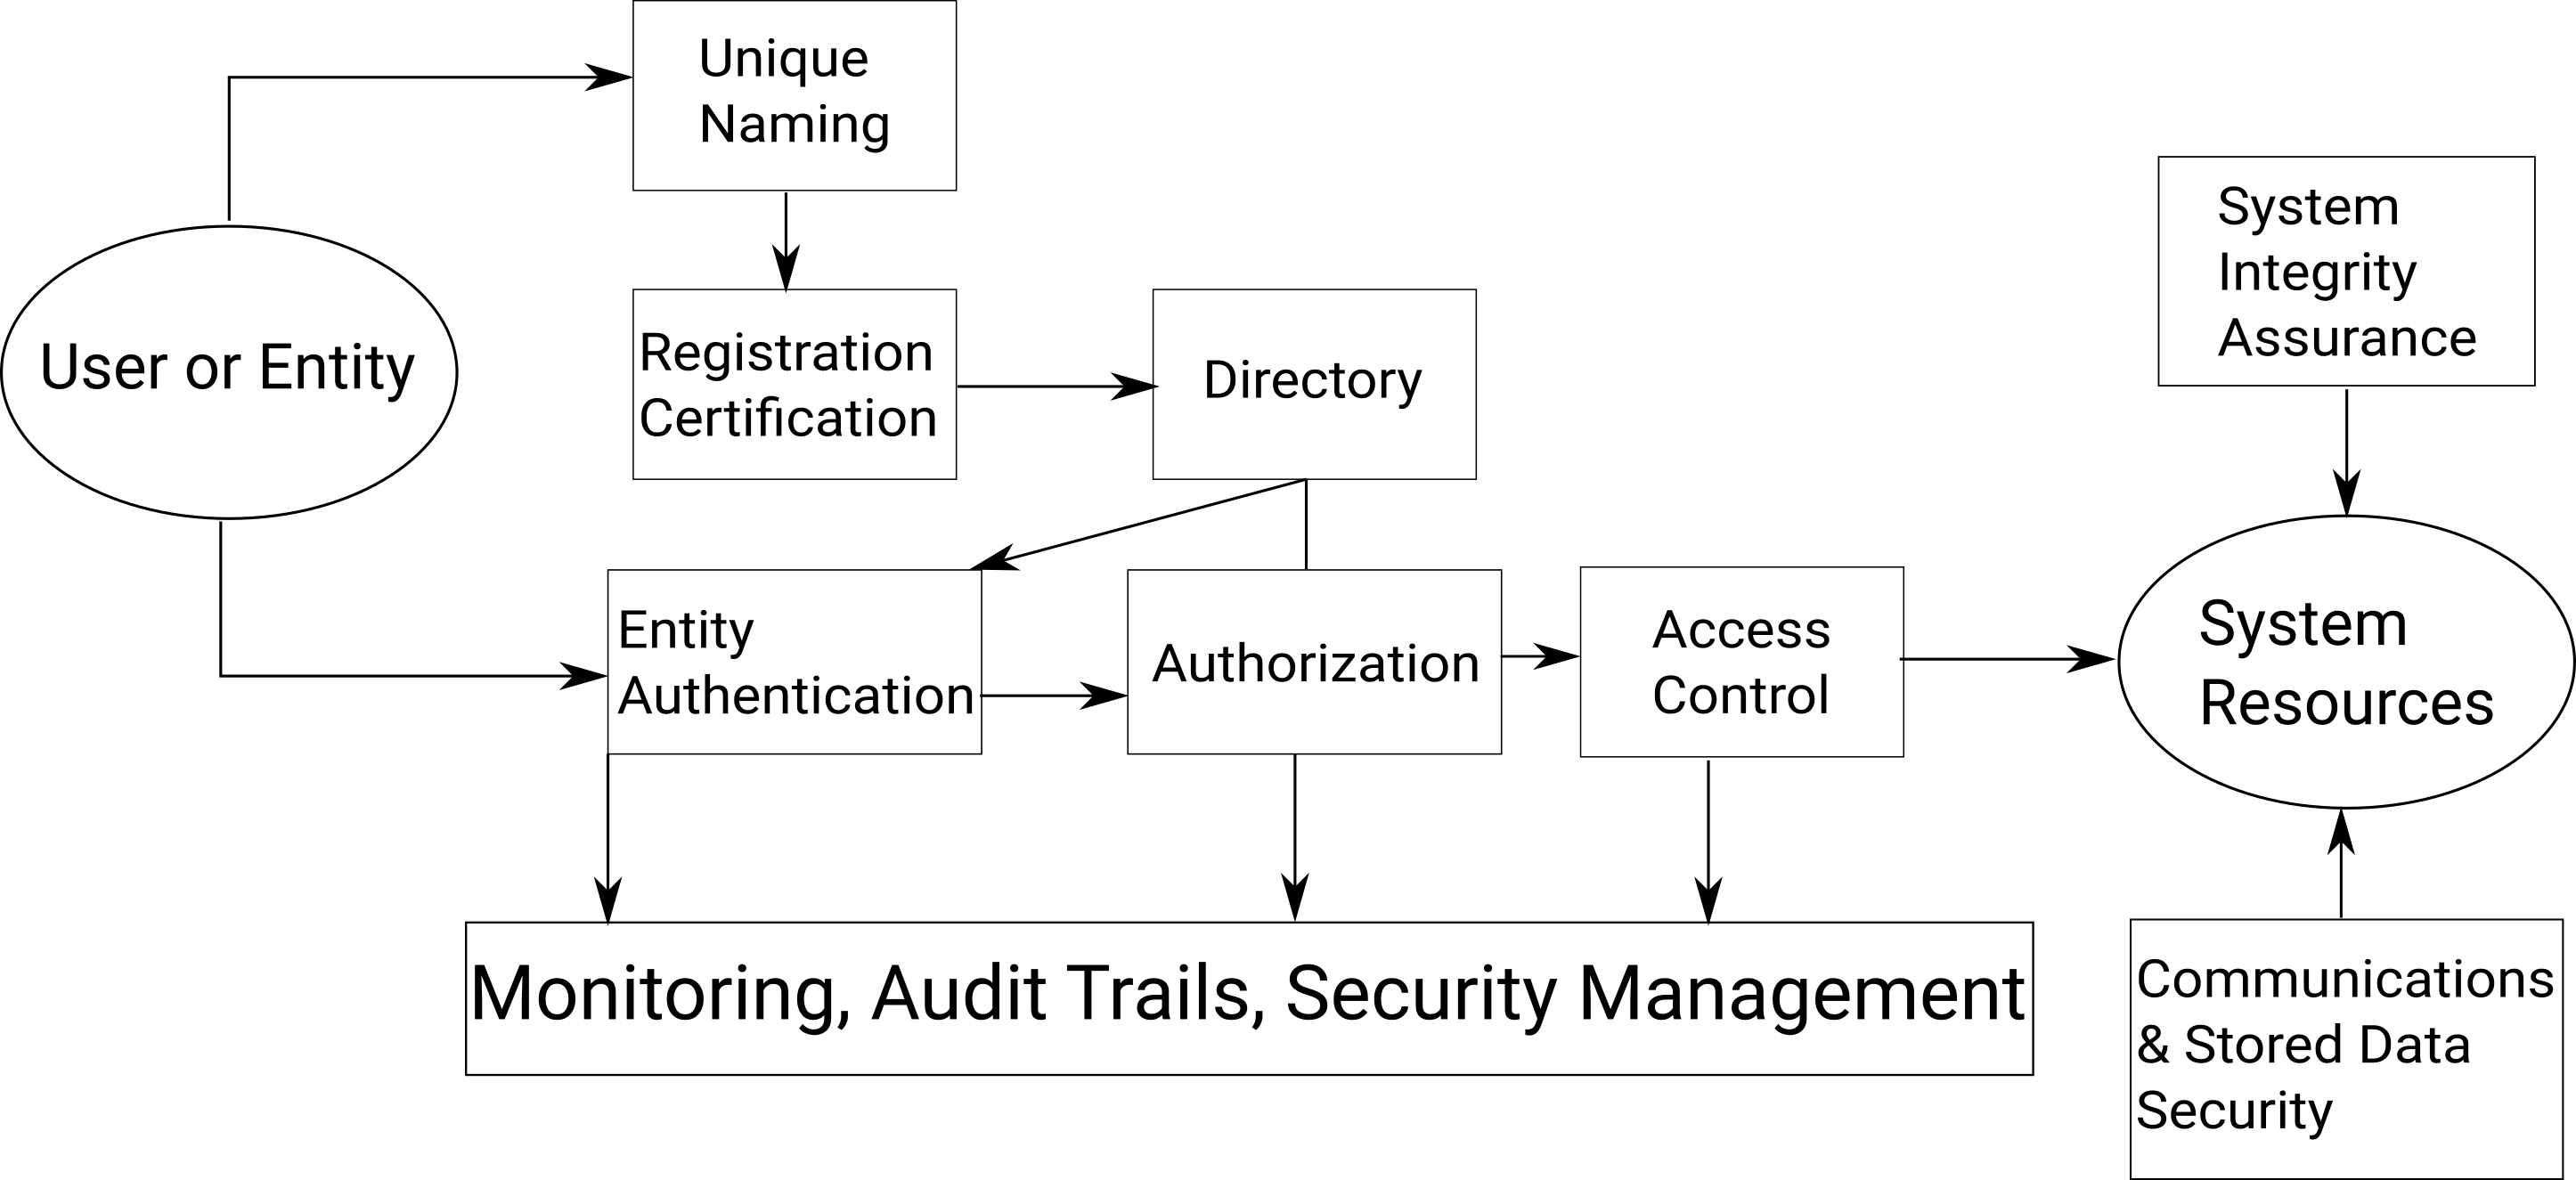
\includegraphics[scale=0.5]{./Drawings/EITP20-Secure_Systems_Engineering/Major_Security_Services_Relations.png}
  \end{solution}

\question{} A logical security architecture can be created using a six steps methodology:
  \begin{parts}
  \part{} Describe each of the different steps
    \begin{solution}
      \begin{enumerate}[noitemsep]
      \item Identify the main entities.
        Here, the users and the physical components in the system(s) are identified.
        Who is doing something and what is executing the user's actions?
      \item Identify the major functions in the system.
        Each computing entity has some function(s) that it needs to fulfill.
        What does each hardware entity need to do?
      \item Identify the security domains and their associations.
        Each entity and function exists within a security domain, i.e.\ how much they are trusted.
        In addition, how do these security domains interact with each other?
      \item Identify security services already meeting the Security Requirements.
        There may be some properties of the system that already meets the requirements as laid out in the Security Requirements.
        Identify these.
        There may also be security services that are required to meed the Security Requirements, identify these too.
      \item Map security services to the functional entities.
        Take the security services from the previous step, and match them together with the entities in the system.
      \item Create a graphical view of the logical architecture.
        It is easier to see how these security services get mapped to the entities and security domains if it is done in a graphical view and their interactions are shown.
        Each computing entity should be a box, each flow of communication an arrow, each user shown, and the computers/users should be grouped together into their security domains.
      \end{enumerate}
    \end{solution}

  \part{} What is the end result?
    \begin{solution}
      A general logical view of the system to see what data needs to be secured and how that should be done.
      This will also specify the security services that should be used, the security domains, the users, the computing entities, among others.
    \end{solution}

  \part{} Give an example of a logical security architecture.
    \begin{solution}
      See Slides 25--31 of Lecture 3.
    \end{solution}
  \end{parts}

\question{} What is a Physical Security Architecture?
  \begin{solution}
    A Physical Security Architecture is the general specification of how to implement the security given by the Logical Security Architecture.
    The expected outcome is a specification of the security solutions offered in the system, including the platform, software, and hardware security functions.
  \end{solution}

\question{} A physical security architecture when using the SABSA includes making a mapping to physical security mechanisms.
  \begin{parts}
  \part{} Describe what is meant by a ``Naming and Registration'' mechanism and give examples.
    \begin{solution}
      The Naming and Registration mechanism is concerned with how we identify the entities within our system.
      Additionally, when they have been given an identifier to recognize by, how we can register them with a system to ensure that when an entity claims to be something with a certain name, we can verify that.

      This typically includes:
      \begin{itemize}[noitemsep]
      \item Unique Naming
        \begin{itemize}[noitemsep]
        \item Using a common naming standard.
        \item Using a common naming procedure.
        \item Using a directory system to separate different names.
        \end{itemize}
      \item Entity Registration
        \begin{itemize}[noitemsep]
        \item Using a standard registration policy.
        \item Having a standard registration procedure.
        \item Using a registration authority system.
        \end{itemize}
      \item Public Key Certification
      \item Directory Services
        \begin{itemize}[noitemsep]
        \item Having a directory system.
        \item Having a directory access protocol.
        \item Having a directory object and attribute syntax rules.
        \item Allowing for directory replication.
        \end{itemize}
      \end{itemize}
    \end{solution}

  \part{} Describe what is meant by a ``Storage and Runtime'' mechanism and give examples.
    \begin{solution}
      This is concerned with how we store data securely and use it securely during runtime.
      \begin{itemize}[noitemsep]
      \item Data confidentiality
      \item Data integrity
      \item Software integrity
      \item Secure Execution
        \begin{itemize}[noitemsep]
        \item Secure hardware modules
        \item Secure execution enclaves
        \item Secure virtual machines
        \item Protected execution
        \end{itemize}
      \item Software licensing Protection
      \item Data and software replication
      \end{itemize}
    \end{solution}

  \part{} Describe what is meant by a ``Physical Security'' mechanism and give examples.
    \begin{solution}
      This is concerned with the physical security of a location.
      \begin{itemize}[noitemsep]
      \item Physical Security
        \begin{itemize}[noitemsep]
        \item Locks on doors
        \item Locked server rooms
        \item Physical protection of cables
        \item Personnel identification
        \end{itemize}
      \item Environmental Security
      \item Personnel Security
        \begin{itemize}[noitemsep]
        \item Background checks
        \item Vetting procedures
        \item Training Courses
        \end{itemize}
      \end{itemize}
    \end{solution}

  \part{} Describe what is meant by an ``Authentication and Session'' protection mechanism and give examples.
    \begin{solution}
      When a registered name wants to access our system, how do we ensure that they are who they say they are and make sure that they have not been compromised?
      \begin{itemize}[noitemsep]
      \item Entity Authentication
        \begin{itemize}[noitemsep]
        \item Login procedure
        \item User passwords/tokens
        \item Authentication protocol
        \end{itemize}
      \item Session Authentication
      \item Message Integrity
        \begin{itemize}[noitemsep]
        \item Message Authentication Codes (MACs)
        \item Hashing
        \end{itemize}
      \item Message Confidentiality
      \item Message Reply Protection
      \item Non-repudiation
      \end{itemize}
    \end{solution}

  \part{} Describe what is meant by a ``User Interface and Naming'' mechanism and give examples.
    \begin{solution}
      Any time a user is interfacing with the system, that is a major vulnerability.
      The user has the ability to doanything they want there, and they may do something that compromises the security of the system.
      So, we need to minimize the number of actions a user can perform on a system to ensure they don't do something that harms the system.
      \begin{itemize}[noitemsep]
      \item User Interface (UI) Security
        \begin{itemize}[noitemsep]
        \item GUI login
        \item GUI Security messages
        \item Single Sign-On
        \end{itemize}
      \item Service Management
      \item Operations Management
      \item Secure Provisioning and Administration
      \end{itemize}
    \end{solution}

  \part{} Describe what is meant by a ``Authorization and Access Control'' mechanism and give examples.
    \begin{solution}
      If an entity is registered, authenticated, and shown to be secure, then what actions do we let them perform, and how can they do them?
      \begin{itemize}[noitemsep]
      \item Authorization
        \begin{itemize}[noitemsep]
        \item Roles
        \item Attributes
        \end{itemize}
      \item Audit Trail
        \begin{itemize}[noitemsep]
        \item Event logs
        \item Logging integrity protection
        \item Log browsing
        \item Log analysis tools
        \end{itemize}
      \item Logical Access Control
        \begin{itemize}[noitemsep]
        \item Access Control Lists (ACLs)
        \item Central Access Manager (CAM)
        \item Access Control Agents
        \item Database Management System
        \item Filesystem management
        \end{itemize}
      \end{itemize}
    \end{solution}

  \part{} Describe what is meant by a ``Monitoring and Incident'' mechanism and give examples.
    \begin{solution}
      When something \textbf{does} go wrong, how can we make sure we find it and know about it?
      \begin{itemize}[noitemsep]
      \item Secure Monitoring
        \begin{itemize}[noitemsep]
        \item User activity logs
        \item Application event logs
        \item Operator activity logs
        \item Management event logs
        \item Event log browsing
        \item Event log analysis
        \item Reporting
        \end{itemize}
      \item Security Measurements and Metrics
        \begin{itemize}[noitemsep]
        \item Cryptographic tests
        \item Inspection tools
        \item Penetration Testing
        \item Statistical Tests
        \end{itemize}
      \item Alarm Management
      \item Intrusion Detection
      \item Incident Response
      \item Disaster Recovery
        \begin{itemize}[noitemsep]
        \item Data and software backups
        \item Data restoration procedures
        \item Hardware redundancy
        \item Recovery plan
        \item Recovery procedure
        \end{itemize}
      \end{itemize}
    \end{solution}
  \end{parts}

\question{} What must in addition to the security mechanisms be specified in the physical security architecture?
  \begin{solution}
    The security of the network and the system's platforms must be considered as well.
  \end{solution}

\question{} Give examples of a platform security solution that can be used to build solutions meeting a logical security service and can be used to protect the chosen physical security mechanism?
  \begin{solution}
    If a logical security service requires secure, unique cryptographic keys be generated, then a platform security solution would be to use a Hardware Security Module to generate them.

    If a logical security service requires something be executed in a hardware-based secure execution environment, then the processor's built-in secure execution environment can be used.
  \end{solution}

\question{} For the SSO logical security architecture given at the lecture, perform the following:
  \begin{parts}
  \part{} Identify the main physical security mechanisms needed in the corresponding physical security architecture.
    \begin{solution}
      \begin{itemize}[noitemsep]
      \item Each user must have a unique naming, likely drawn from their legal name.
      \item Each user must have a device(s) registered to them, which must be tracked.
      \item Each device will have keys to be able to use the system.
      \item The user has a password to be able to user the Single-Sign On service.
      \item The OIDC client must perform an authentication action on the user.
      \item The OIDC client must then confirm the authenticity of the user with the OIDC provider.
      \item This must them go to the Hosting Servers to perform the actual computation.
      \item Each of these servers must have replicas ready to take over.
      \item Each of these servers must also have data backups, in case of failure.
      \item They must be stored somewhere separate from the physical location of the user, likely close to the services that the SSO service provides.
      \item The physical security of this location must be tested.
      \item The UI for signing in should be as simple as possible.
      \item Once the user signs in, they should not have to do it again. If the system requires them to ``sign in'' again, then there needs to be a button for SSO.\@
      \item All login attempts should be logged, with user- and device-identifying information recorded too.
      \item There needs to be monitoring to ensure inappropriate IP addresses are banned (Users obviously not from your group).
      \end{itemize}
    \end{solution}

  \part{} Identify the main platform security components needed to fulfill the architecture
    \begin{solution}
      \begin{itemize}[noitemsep]
      \item The system must have a user database somewhere.
      \item The user's passwords are only stored in their final hashed value.
      \item The servers and databases must have replicas for failover, and backups for complete failure.
      \item Any actions these servers take must be logged with entity-identifying information.
      \item Unlikely we need HSMs to generate keys, use built-in cryptographic functions on devices.
      \item Run the minimum of services required for functioning.
      \item The servers that run identification should likely run in a hardware-based secure execution environment.
      \item Each of these servers could be VMs as well, to allow for on-demand scaling and to prevent one issue from propagating.
      \end{itemize}
    \end{solution}

    \begin{subparts}
    \subpart{} Suggest concrete platform security mechanisms to use for the physical realization.
    \end{subparts}
  \end{parts}
\end{questions}

%%% Local Variables:
%%% mode: latex
%%% TeX-master: "../EITP20-Secure_Systems_Engineering-Study_Questions"
%%% End:
